\documentclass[pdftex,12pt,letter]{article}

\usepackage{graphicx}
\usepackage{placeins}
\usepackage{enumerate}
\makeatletter
  \renewcommand\@seccntformat[1]{\csname the#1\endcsname.\quad}
\makeatother
\newcommand{\HRule}{\rule{\linewidth}{0.5mm}}
\begin{document}

\begin{titlepage}
\begin{flushright}
\HRule \\
{\huge \bfseries Case Scheduler\\[4cm]}
{\large Prepared by\\Jason Kuster, Stuart Long, and Nathan McKinley\\[1cm]
October 29, 2012}
\end{flushright}
\end{titlepage}
%\tableofcontents{}
%\newpage
\section*{Introduction Overview}
Currently, there only exist functional but not particularly elegant ways for students to visualize their class schedules. For our project, we want to make a better Case Scheduler, one which works fast and is easy for students to use.\\

\noindent When making a class schedule, it is very helpful to be able to see what your schedule looks like. The two systems currently available, SIS and scheduler.case.edu do an unsatisfactory job of displaying the schedule. The problem with SIS is that it's exceedingly slow and inefficient for course planning, and is much more suited to only doing course enrollment. The problem with scheduler.case.edu is that not only is it slow to open and do anything, but it is impossible to print without using the Print Screen function on your computer, exporting it to an image, and printing that image. In addition, there are many expansions which could be made to functionality, such as easy sharing of schedules and planning your schedule with friends. What we plan to do is to duplicate the functionality of the current Case Scheduler, while completely rewriting the user interface and backend code to allow for a better user experience.\\

\noindent We will be using two technologies to implement this scheduler. First, we will be using Python and the Django framework for programming our web application. Second, we will be using MySQL for our database.
\section*{Application Requirements Specifications}
\begin{enumerate}[1.]
\item The system will maintain a per-user list of courses.\\\\
This is the main focus of our project. Our object is to create a place to which students are able to come and put in and plan their schedule. In order for this to happen, we must maintain per-user lists of courses. These lists of courses will be maintained for four years, after which point they will be discarded. We will allow for creation of lists for the current semester, as well as the next semester once the data is available from the Student Information System.
\item The system will allow the user to search the catalog for courses.\\\\
In order to create their lists of courses, users must be able to find the courses they wish to take. Our system will support searching by course name and will match queries based on course name, description, and instructor. The search results will be displayed in a convenient list view, with the differences clearly marked (course name, meeting time, instructor, etc). The current Case Scheduler view is shown below.\\
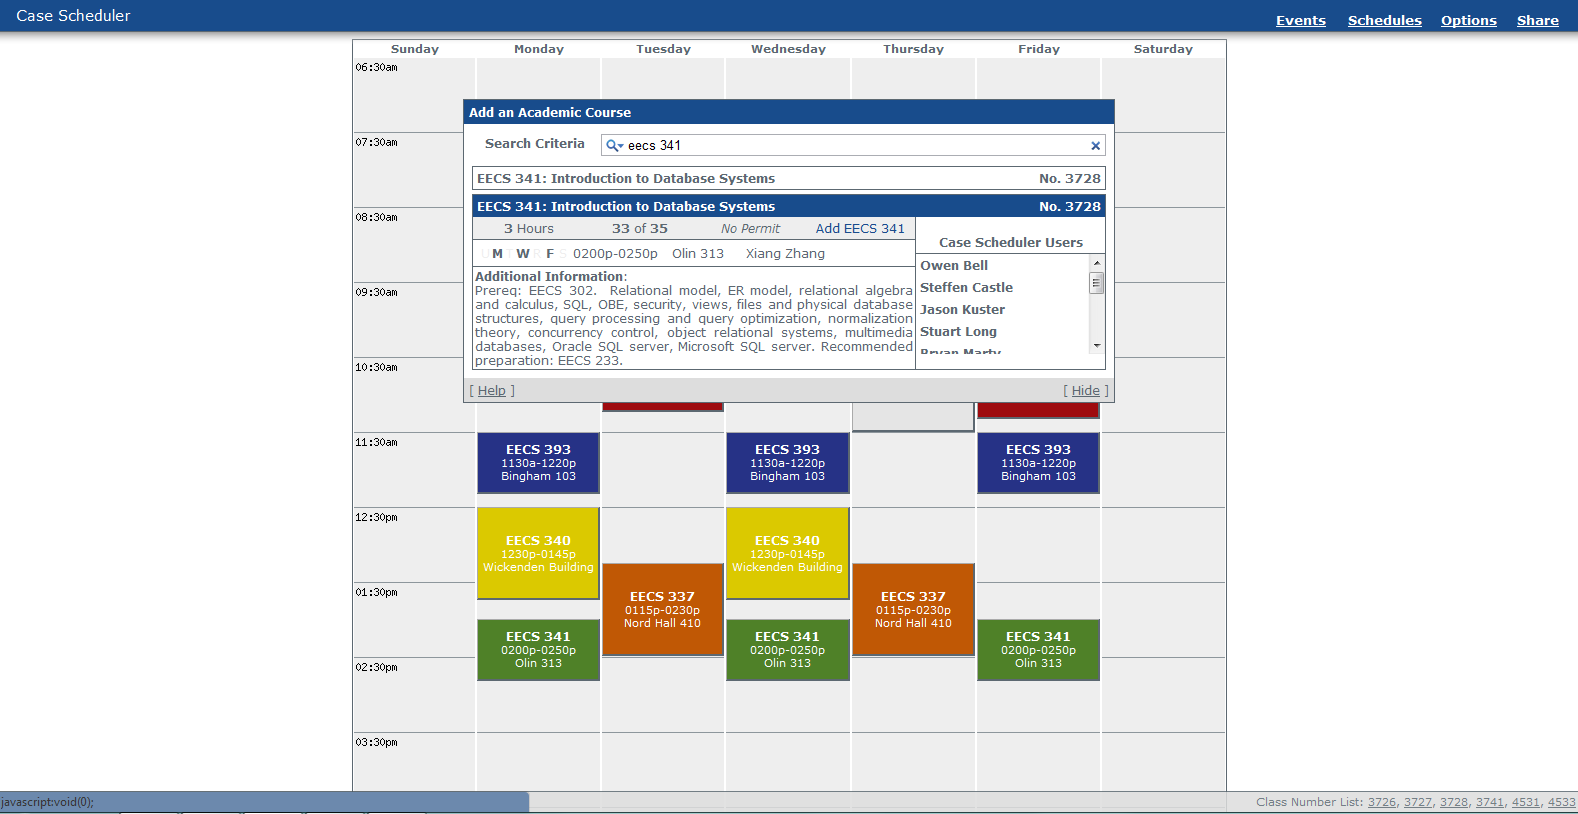
\includegraphics[width=130mm]{add_course.png}
\item The system will allow courses to be added to users' active schedule.\\\\
Once found, a course must be able to be added to a user's currently active schedule. It should stay there until removed either by them or by the system. The functionality of this will be very similar to the functionality of the current Case Scheduler, as shown in the above graphic, but will have a reworked user interface designed by our team.
\item The system should support removing a course from a particular schedule.\\\\
As a user's courses can change during the planning stages or during drop/add, users should be able to remove courses which they have added from their lists.
\item The system will display course information on a weekly calendar-formatted schedule, including course name, times, instructor, and location.\\\\
This format seems to be the easiest and most convenient to view, and gives users a quick and easy-to-use overview of their courses for the week. In the future, other layouts such as a list-type view, day-by-day view, and monthly view. Our implementation of the weekly view will look similar to the below graphic, although with a rewritten user interface backend.\\
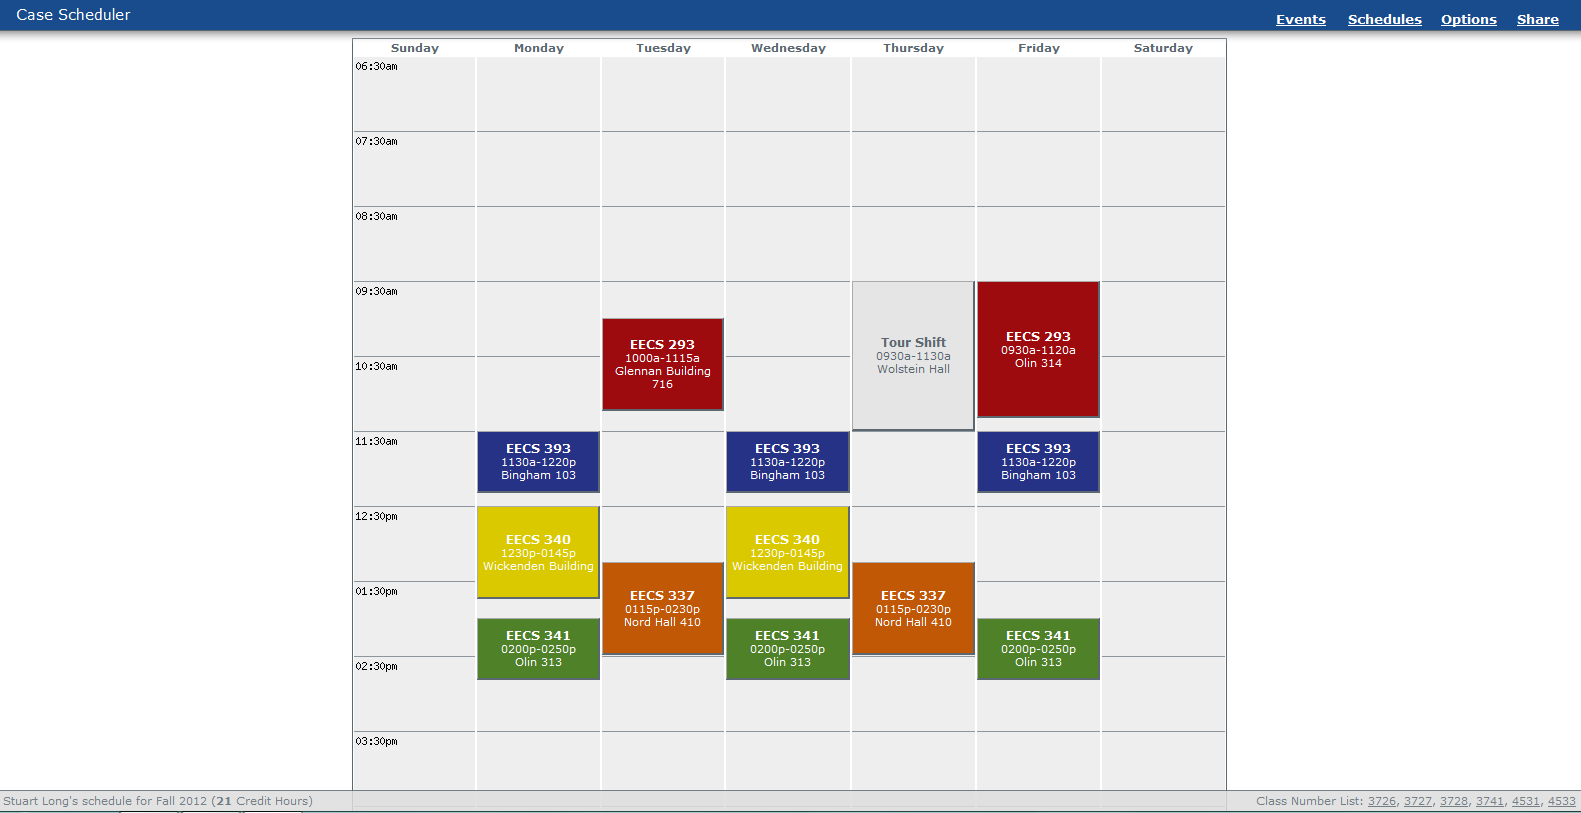
\includegraphics[width=130mm]{main_schedule.png}
\item The system should display itself in a manner which facilitates printing.\\\\
The current system makes it exceedingly difficult to print one's schedule. We are making sure that by design our system will be formatted for printing without users having to do anything.
\item The system should maintain users' lists across SIS updates.\\\\
As the list of courses is subject to change as courses are added or removed in SIS, we will make sure that our application remains robust across these changes and that when responding to changes in the schedule of classes xml file, we do not inadvertently break anyone's schedule.
\item Clicking on courses will bring up more detailed course information.\\\\
As there is a wealth of information about the courses in SIS, we plan to make that data consumable by our users by adding a detail page to each course. This detail page will include such items as classroom, teacher, and meeting times, among others.
\item Under reasonable load, the system should have loading times of less than one second.\\\\
At the current time, scheduler.case.edu can take upwards of 15 seconds to properly aggregate and display all of a user's classes. This frustrates users and is a design flaw which should be easily remediable. Our system will have much faster response times, ensuring greater user satisfaction and a more usable product.
\item The system will allow users to change their current working semester, and will maintain schedules up to 4 years in the past.\\\\
This is necessary in order to allow users to plan a next semester while having a schedule for their current semester. The second SIS data is available, we will make it available to the students and allow them to start planning their next semester. In addition, the ability to go and see what courses they have taken in previous semesters provides value because students will no longer have to do the time-consuming process of using SIS.
\item The system supports the creation of custom events.\\\\
In order to be a one-stop schedule manager, as well as to remain more feature-complete than the current case scheduler, we will be adding support for custom events such as TA sessions, jobs, and other user-defined events. These custom events will have all of the behavior of courses, but will be visible only to their creator, i.e they will not appear in searches. The add dialog will look similar to below.\\
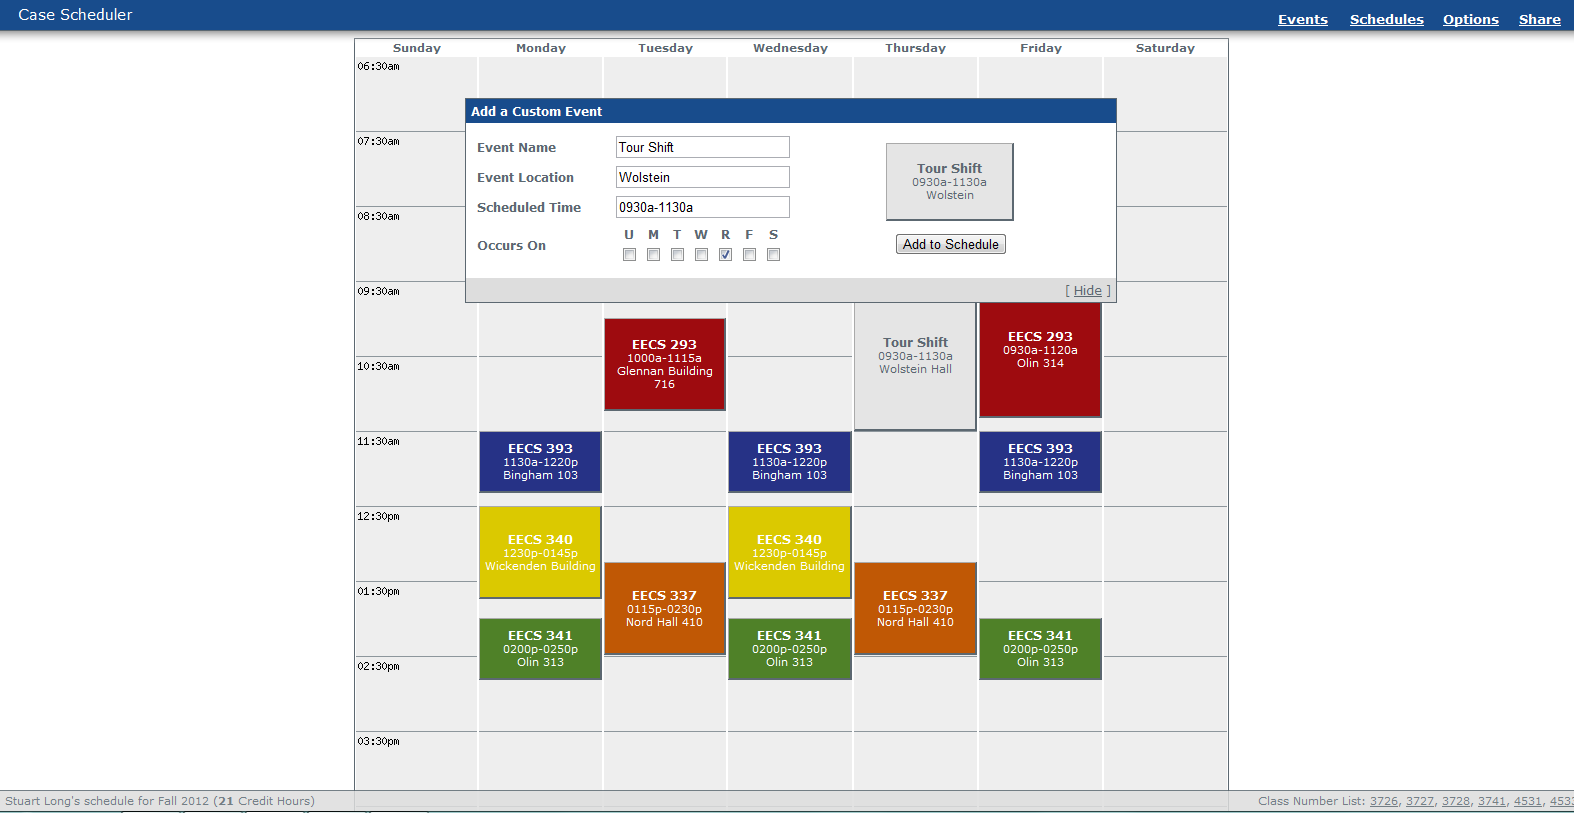
\includegraphics[width=130mm]{add_event.png}
\end{enumerate}
\section*{Database Requirements Specifications}
\subsection*{Objects and Relationships}
\begin{enumerate}[1.]
\item Course Offering: The database will have an instance of course offering for each course offered by CWRU. Every course offering is-a course, which is described below. This entity it important to our application because a course offering is the typical item that a user will actually had to his or her schedule. A course offering will have at least the following attributes: offering id, term, subject, status, dates, days/times, room, total capacity, current enrollment, and description.\\\\  In explanation, the "component" attribute represents the type of the course, whether it's a lecture, recitation, or similar. The "status" attribute represents whether the course is  open, closed, or other, which is important for a user to know when scheduling for a certain course. "Current Enrollment" signifies how many other students are registered for the course offering. "Description" is a paragraph explanation of the course provided by the department or professor, also important info for a user browsing through various courses.
\item Course: every course offering is-a course. A course entity is useful to have for this application because it will allows the application to more easily display all of the course offering for a selected course. The course entity will have the following attributes: title, catalog number, component, units (max), and label. In explanation, the "label" attribute corresponds to a short combination of the of the subject, catalog number, and title. The catalog number corresponds to the course number within that courses department (e.g. 314 for EECS 341). Courses will also have prerequisite as specified by the Has\_Prerequisite relationship, detailed below.
\item Has\_Prerequisite Relationship: This relationship involves only Course entities. Any one course may have multiple prerequisites and may be a prerequisite for multiple courses. This relationship will allow the application to easily display and direct users to what prerequisites a given course may have.
\item User: Every user will log onto our application with their case id and password (using the single sign on service as provided by CWRU). This process allows us to keep an object representation of each user. This application doesn't need much information about each user, so it will just keep track of the user's case id and last login date. We keep track of their login date so we can safely delete a user and any relationships that user participated in after the user has not logged in for four years.
\item Instructor: Our application will allows users to find basic information about CWRU instructors, such as office location, office hours, and contact information. To adequately display this information, the instructor object will have at least the following attributes: instructor ID, office location, office hours, phone number, and email.
\item Teaches Relationship: Every course offering will be taught by an instance of instructor, and this relation models that, simply by storing the id's for the course offering and the instructor that teaches it. We assume a course offering is not taught by more than one instructor, an assumption that is sufficient for a scheduling application.
\item Enrolled-in Relationship: Multiple students can take multiple different courses, and courses can have many students enrolled in it, up to that courses capacity. This relationship is fairly simple in that it just keeps track of a student and a course that student is enrolled in. However, it is also an extremely important relationship because it allows us to populate a students schedule.
\item Custom Event: Like the current Case Scheduler, our application will allow users to add their own recurring custom events to the schedule. A good example might be an extra-curricular actives such as band rehearsals or sport practices. As such, the databases needs a separate entity to store these events. This entity will have the following attributes: days/times, location, title, semester, and description. This entity will be a weak entity and each custom event will be connected to a single user through the Has relationship.
\item Has Relationship: The Has relationship, again, connects users to the custom events they have created. This relationship is a one-to-many relationship, so a user may have many custom events, and it requires full participation on the part of the custom event entities.
\end{enumerate}
\subsection*{Queries and Transactions}
\begin{enumerate}[1.]
\item Get\_List:  Since the application is centered around displaying a graphical representation of a list of courses, we will need to retrieve the list of courses associated with the current user.  Since we will not be storing this list in cookies, we will need to retrieve it from the database every time we seek to display it.  This will be required approximately once per page-view.  This will require as input the user ID (Case ID), and produce as output a list of course ids.
\item Lookup\_Course:  Since the application will need to display information about each course in the list of courses, we will need to retrieve this information.  This information will include things like course title, course description, instructor, course time, and course location.  Since most lists will contain more than one course, we will need to perform this query more than one time per page view.  This query will require as input a course ID, and will return several columns which will be used to build the calendar.
\item Add\_Course:  Since the application requires that a user build a list of courses, the user will be need to be able to build the list of courses by adding to it.  We will add courses to the user lists using this transaction.  This transaction will take as input the user ID and a course ID and will add the course ID to the list of courses for the user in question.  It will not return anything.  This will be done much less than once per page view, since the average user will need to view their courses more than once, but will only need to add them one time each.
\item Remove\_Course:  The opposite of Add\_Course, sometimes users will need to remove courses that they've already added.  This will happen even less often than Add\_Course, because most users will only add courses that they plan to view in the future.  Most users do not drop courses, and so most users will only need to add courses.  This will happen far less than once per page view.  This transaction will take as input the User ID and Course ID, and will delete the row from the table pairing users and courses, and will not return anything.
\item Lookup\_Instructor:  One feature that users might desire is the ability to lookup all courses that a particular instructor is teaching.  This means that we will want to index the courses table by instructor as well as by course ID.  This query will be used much less frequently than the other queries and transactions because the primary feature of the application is display of a calendar, not viewing the courses taught by a particular instructor.  This transaction will take as input the instructor name, and will return a list of course IDs taught by that instructor.
\item Create\_Event: Users will be allowed to create their own custom events to add to any schedule they desire. The application will use the event's semester attribute to determine which schedule to add the event to.
\end{enumerate}
\subsection*{Actions and Events}
\begin{enumerate}[1.]
\item This application will display users' schedules based on the currently selected semester, with the default semester being the current semester at the time of the user login. The application will have a drop down list or similar form that will allow users' to select any other schedule in which the user has a course. As can be seen above, the database does not have an actual "schedule" object. To craft various semester schedules, the course offering relations will just be queried for term and the user's schedules will be constructed off of that. All of a user's schedules will be stored until that user is deleted, see \textit{Integrity Constraints} for user deletion policies.
\item An event that will happen every time the application is used by any user is a user login. To use this application a user must have a CWRU ID and password, and will log in with the CWRU Single Sign-On Service. By logging in, the application will be able to identify the user and load all of that user's schedules.
\end{enumerate}
\subsection*{Integrity Constraints}
\begin{enumerate}
\item Users must be enrolled in at least one course offering. If, for some reason, a user is no longer enrolled in any course offering, then that user is removed from the database. If the user wants to use an application after being deleted, than a new "user" object for that user will be created upon log-in, as if that user was a first time user.
\item This application may have to handle up to all CWRU community members and several schedules per user. In order to maintain a flexible ceiling on the database, users that have been inactive for more than four years. If a user is removed and one of the course offerings that that user was enrolled in no longer has any users enrolled in it, then that course offering is deleted as well.
\item If, at any time, a course offering has no users enrolled in it, and the current semester is after the semester that course offering took place in, then that course offering will be removed.
\item Instructors are allowed to not teach a course offering at any given time. However, if an instructor continuously does not teach a course for five years, then that instructor is removed.
\item Every custom event must be involved in a Has relationship with some user.
\item Every course offering must satisfy the is-a course relationship.
\end{enumerate}
\section*{ER Diagram}
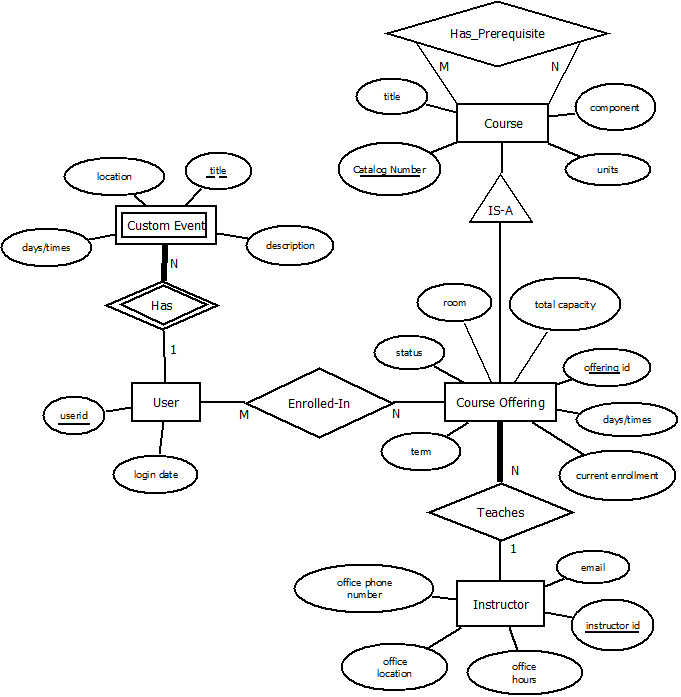
\includegraphics[width=120mm]{ERDiagram.png}
\FloatBarrier
\pagebreak
\section*{Relational Model}
\begin{verbatim} 
CREATE_TABLE User
  (userid CHAR(6),
  login date CHAR(10) NOT NULL,
  PRIMARY KEY (userid))
  
CREATE_TABLE CustomEvent
	(userid CHAR(6) NOT NULL,
	days/times CHAR(20),
	location CHAR(40),
	title CHAR(40),
	semester CHAR(12),
	description CHAR(120),
	PRIMARY KEY (userid, title, semester)
	FOREIGN KEY (userid) REFERENCES User
		ON DELETE CASCADE

CREATE_TABLE Enrolled_In
  (userid CHAR(6),
  coid CHAR(8),
  PRIMARY KEY (coid, userid),
  FOREIGN KEY (userid) REFERENCES User,
      ON DELETE CASCADE
  FOREIGN KEY (coid) REFERENCES CourseOffering,
      ON DELETE CASCADE)
      
CREATE_TABLE CourseOffering
  (coid CHAR(8),
  status CHAR(20),
  room	CHAR(20),
  total_capacity INTEGER,
  days/times CHAR(20),
  current_enrollment INTEGER,
  term CHAR(16),
  description CHAR(400),
  instructorId CHAR(8) NOT NULL,
  catalogNumber CHAR(12) NOT NULL,
  PRIMARY KEY (coid),
  FOREIGN KEY (instructorId) REFERENCES Instructor
  		ON DELETE CASCADE
  FOREIGN KEY (catalogNumber) REFERENCES Course
  		ON DELETE CASCADE
  		
CREATE TABLE Course
	(catalogNumber CHAR(12),
	title CHAR(40),
	component CHAR(20),
	units REAL,
	PRIMARY KEY (catalogNumber))
	
CREATE TABLE Has_Prerequisite
	(prereqCnumber CHAR(12),
	prereqForCnumber CHAR(12),
	PRIMARY KEY (prereqForCnumber, prereqCnumber),
	FOREIGN KEY (prereqForCnumber) REFERENCES Course
		ON DELETE CASCADE
	FOREIGN KEY (prereqCnumber) REFERENCES Course
		ON DELETE CASCADE)
		
CREATE TABLE Instructor
	(instructorId CHAR(8),
	email CHAR(20),
	officeHours CHAR(20),
	officeLocal CHAR(20),
	phoneNumber INTEGER)
  \end{verbatim}
\subsection*{Justification of Relational Model}
\begin{itemize}
\item User HAS Custom Event (1:N, full participation from Custom Event to Has)
\subitem This relationship is satisfied by two pieces: first, the Custom Event has a key for the id of the user to which it is attached. This satisfies the 1:N part of the relationship. Second, the id is listed as NOT NULL, which enforces the full participation.
\item User Enrolled-In Course Offering (M:N)
\subitem This relationship is satisfied by the inclusion of the Enrolled-In table, which contains a user id and an offering id.
\item Instructor Teaches Course Offering (1:N, full participation from Instructor to Course Offering)
\subitem This relationship is satisfied by two pieces: first, each Course Offering has an Instructor id key corresponding to the instructor who teaches the class. This satisfies the 1:N part of the relationship. The full participation from Course Offering to Teaches is enforced by the NOT NULL on the Instructor ID.
\item Course Offering IS-A Course
\subitem The IS-A relationship here is satisfied by having each Course Offering contain a catalog number, which connects it to a specific instance of a course. It thus becomes an instance of that course.
\item Course Has\_Prerequisite
\subitem The Has\_Prerequisite relationship is satisfied by the inclusion of the Has\_Prerequisite table. It contains two keys, one key for the course in question, and another for the course for which it is a prerequisite. In this way, one course can have multiple prerequisites and can also be a prerequisite for multiple classes.
\end{itemize}
\section*{Installing on a DBMS}
We successfully installed mysql on a linux machine that one of our group members owns.  The machine is running Ubuntu, so the installation was a very straightforward process.  We simply ran 'apt-get install mysql-server'.  After that, we needed to create the scheduler database, which was done simply:\\\\
\begin{verbatim}
CREATE DATABASE scheduler;
USE scheduler;
\end{verbatim}

Then it got fairly complicated.  It became apparent (see figure 1) that the syntax we've been using wasn't correct.  In mysql, foreign key constraints need to be declared after the keys themselves; in the SQL we learned, they could be declared at the end of the CREATE TABLE statement.  This correction was necessary throughout the set of table creations.  About halfway through it became clear how the SQL needed to be modified.  We then used DESCRIBE calls to ensure that everything was set up correctly.
\begin{flushleft}
\begin{figure}
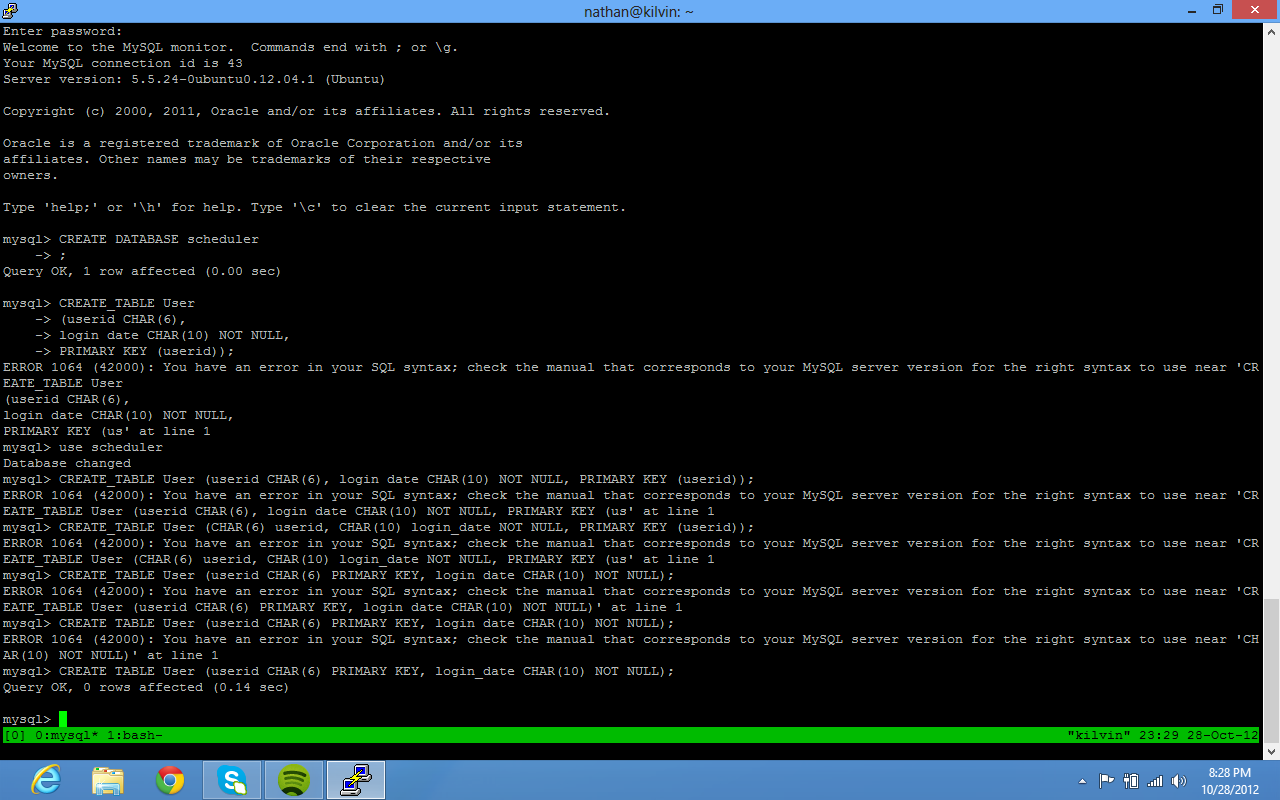
\includegraphics[width=140mm]{db1.png}
\figurename{ 1}
\end{figure}
\begin{figure}
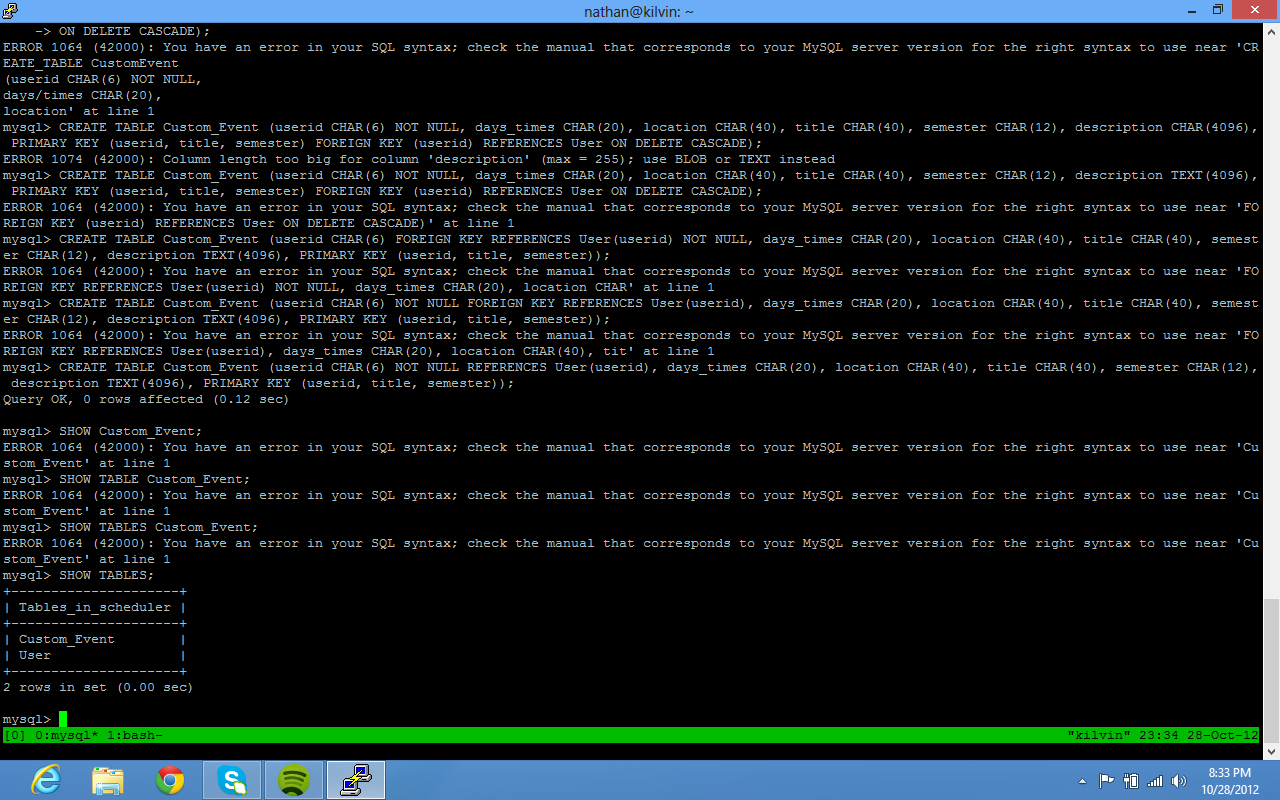
\includegraphics[width=140mm]{db2.png}
\figurename{ 2}
\end{figure}
\begin{figure}
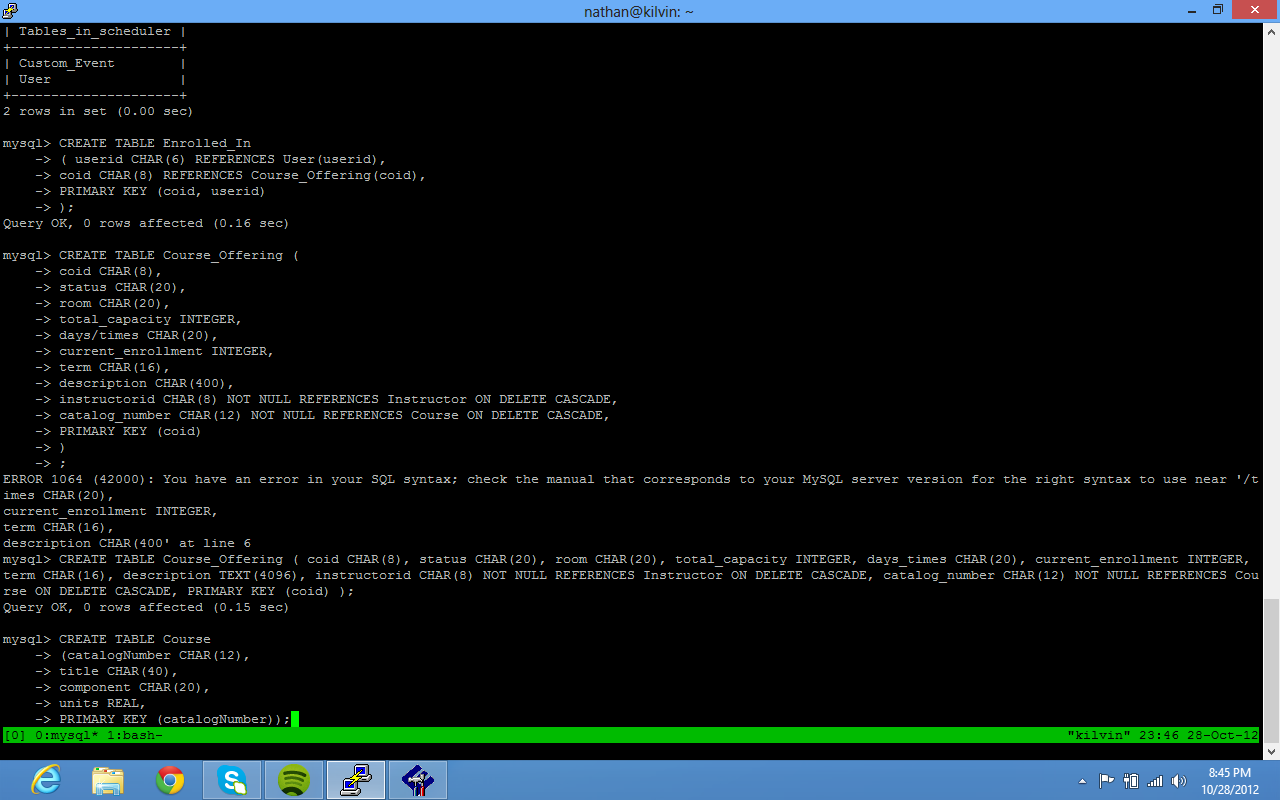
\includegraphics[width=140mm]{db3.png}
\figurename{ 3}
\end{figure}
\begin{figure}
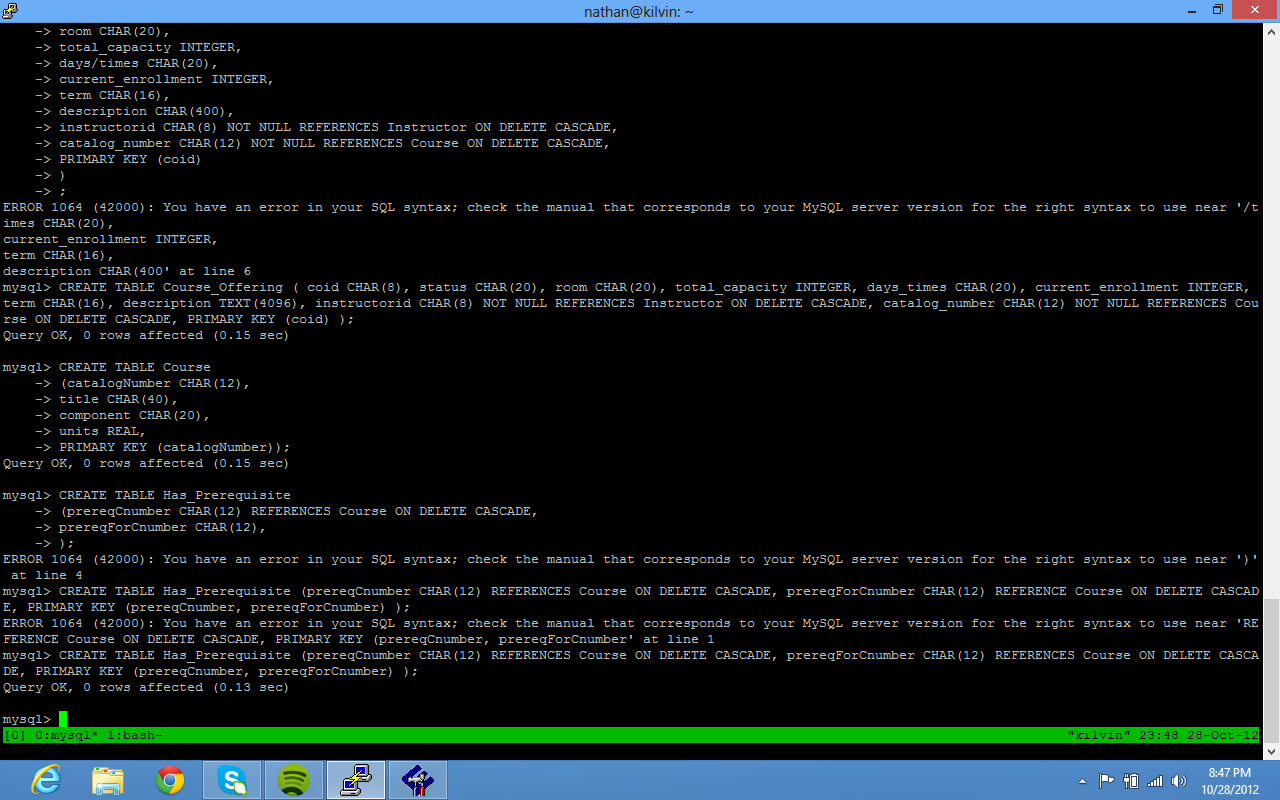
\includegraphics[width=140mm]{db4.png}
\figurename{ 4}
\end{figure}
\begin{figure}
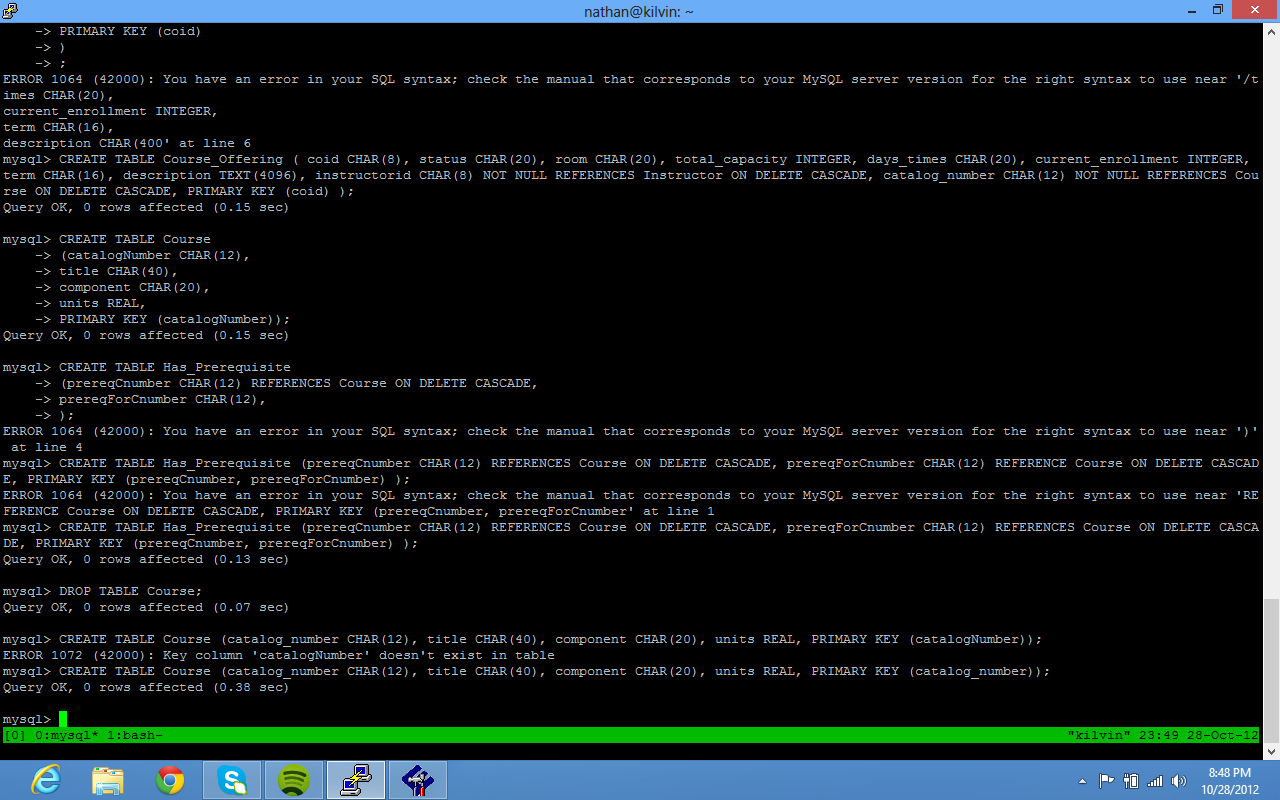
\includegraphics[width=140mm]{db5.png}
\figurename{ 5}
\end{figure}
\begin{figure}
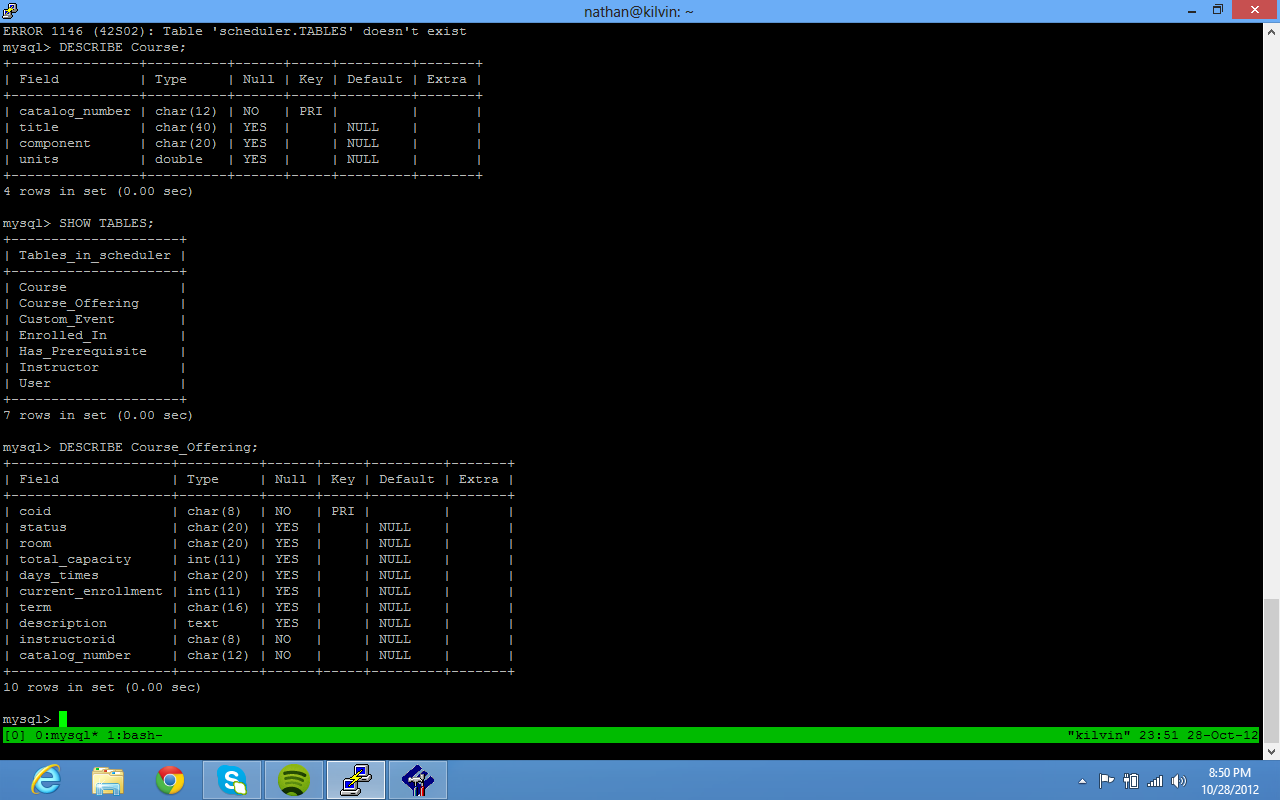
\includegraphics[width=140mm]{db6.png}
\figurename{ 6}
\end{figure}
\begin{figure}
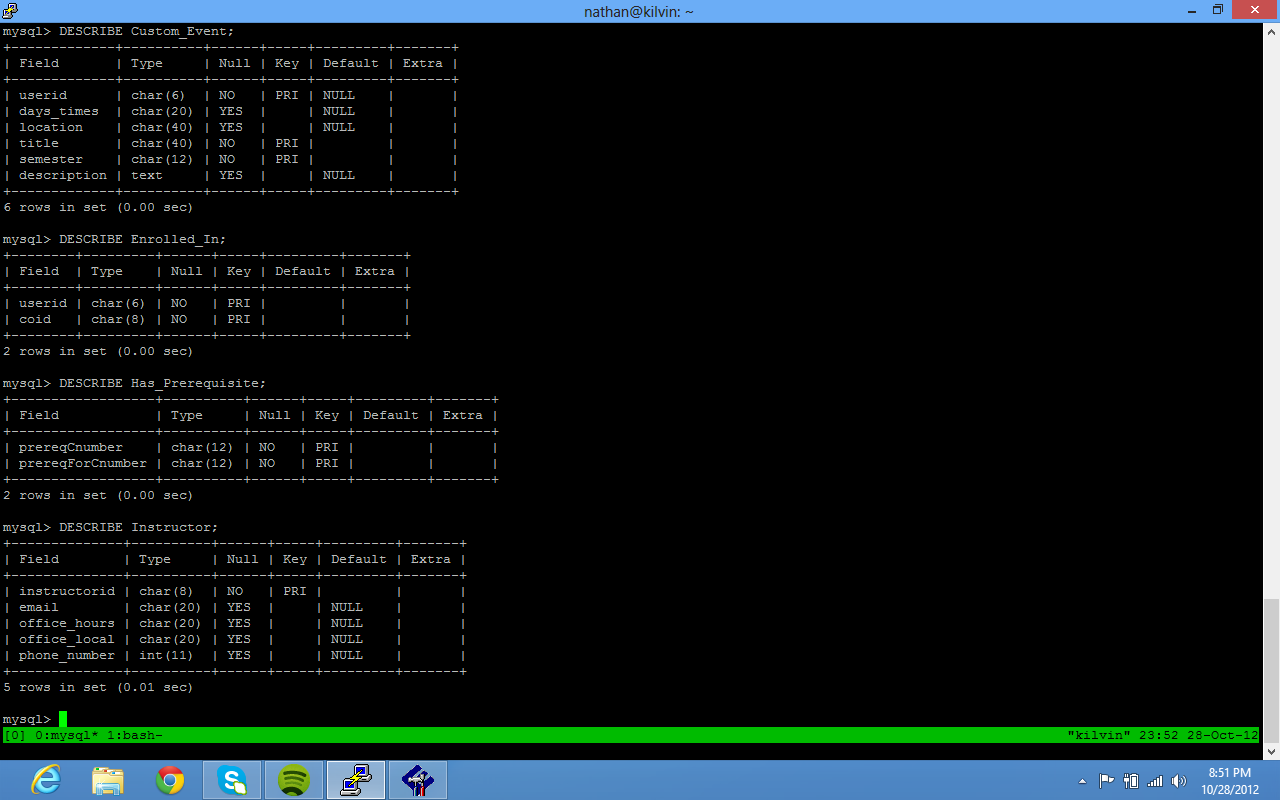
\includegraphics[width=140mm]{db7.png}
\figurename{ 7}
\end{figure}
\begin{figure}
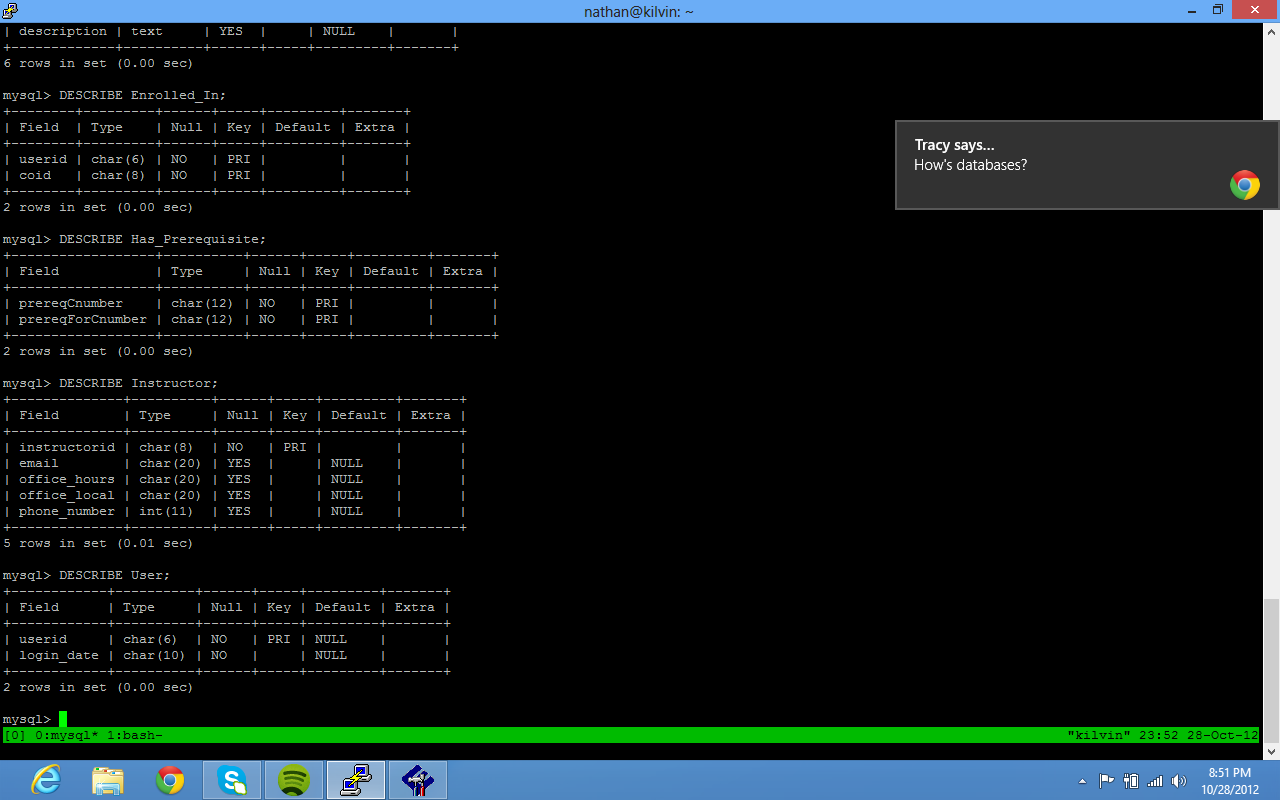
\includegraphics[width=140mm]{db8.png}
\figurename{ 8}
\end{figure}
\end{flushleft}
\end{document}
